% Options for packages loaded elsewhere
\PassOptionsToPackage{unicode}{hyperref}
\PassOptionsToPackage{hyphens}{url}
%
\documentclass[
]{article}
\usepackage{amsmath,amssymb}
\usepackage{iftex}
\ifPDFTeX
  \usepackage[T1]{fontenc}
  \usepackage[utf8]{inputenc}
  \usepackage{textcomp} % provide euro and other symbols
\else % if luatex or xetex
  \usepackage{unicode-math} % this also loads fontspec
  \defaultfontfeatures{Scale=MatchLowercase}
  \defaultfontfeatures[\rmfamily]{Ligatures=TeX,Scale=1}
\fi
\usepackage{lmodern}
\ifPDFTeX\else
  % xetex/luatex font selection
\fi
% Use upquote if available, for straight quotes in verbatim environments
\IfFileExists{upquote.sty}{\usepackage{upquote}}{}
\IfFileExists{microtype.sty}{% use microtype if available
  \usepackage[]{microtype}
  \UseMicrotypeSet[protrusion]{basicmath} % disable protrusion for tt fonts
}{}
\makeatletter
\@ifundefined{KOMAClassName}{% if non-KOMA class
  \IfFileExists{parskip.sty}{%
    \usepackage{parskip}
  }{% else
    \setlength{\parindent}{0pt}
    \setlength{\parskip}{6pt plus 2pt minus 1pt}}
}{% if KOMA class
  \KOMAoptions{parskip=half}}
\makeatother
\usepackage{xcolor}
\usepackage[margin=1in]{geometry}
\usepackage{color}
\usepackage{fancyvrb}
\newcommand{\VerbBar}{|}
\newcommand{\VERB}{\Verb[commandchars=\\\{\}]}
\DefineVerbatimEnvironment{Highlighting}{Verbatim}{commandchars=\\\{\}}
% Add ',fontsize=\small' for more characters per line
\usepackage{framed}
\definecolor{shadecolor}{RGB}{248,248,248}
\newenvironment{Shaded}{\begin{snugshade}}{\end{snugshade}}
\newcommand{\AlertTok}[1]{\textcolor[rgb]{0.94,0.16,0.16}{#1}}
\newcommand{\AnnotationTok}[1]{\textcolor[rgb]{0.56,0.35,0.01}{\textbf{\textit{#1}}}}
\newcommand{\AttributeTok}[1]{\textcolor[rgb]{0.13,0.29,0.53}{#1}}
\newcommand{\BaseNTok}[1]{\textcolor[rgb]{0.00,0.00,0.81}{#1}}
\newcommand{\BuiltInTok}[1]{#1}
\newcommand{\CharTok}[1]{\textcolor[rgb]{0.31,0.60,0.02}{#1}}
\newcommand{\CommentTok}[1]{\textcolor[rgb]{0.56,0.35,0.01}{\textit{#1}}}
\newcommand{\CommentVarTok}[1]{\textcolor[rgb]{0.56,0.35,0.01}{\textbf{\textit{#1}}}}
\newcommand{\ConstantTok}[1]{\textcolor[rgb]{0.56,0.35,0.01}{#1}}
\newcommand{\ControlFlowTok}[1]{\textcolor[rgb]{0.13,0.29,0.53}{\textbf{#1}}}
\newcommand{\DataTypeTok}[1]{\textcolor[rgb]{0.13,0.29,0.53}{#1}}
\newcommand{\DecValTok}[1]{\textcolor[rgb]{0.00,0.00,0.81}{#1}}
\newcommand{\DocumentationTok}[1]{\textcolor[rgb]{0.56,0.35,0.01}{\textbf{\textit{#1}}}}
\newcommand{\ErrorTok}[1]{\textcolor[rgb]{0.64,0.00,0.00}{\textbf{#1}}}
\newcommand{\ExtensionTok}[1]{#1}
\newcommand{\FloatTok}[1]{\textcolor[rgb]{0.00,0.00,0.81}{#1}}
\newcommand{\FunctionTok}[1]{\textcolor[rgb]{0.13,0.29,0.53}{\textbf{#1}}}
\newcommand{\ImportTok}[1]{#1}
\newcommand{\InformationTok}[1]{\textcolor[rgb]{0.56,0.35,0.01}{\textbf{\textit{#1}}}}
\newcommand{\KeywordTok}[1]{\textcolor[rgb]{0.13,0.29,0.53}{\textbf{#1}}}
\newcommand{\NormalTok}[1]{#1}
\newcommand{\OperatorTok}[1]{\textcolor[rgb]{0.81,0.36,0.00}{\textbf{#1}}}
\newcommand{\OtherTok}[1]{\textcolor[rgb]{0.56,0.35,0.01}{#1}}
\newcommand{\PreprocessorTok}[1]{\textcolor[rgb]{0.56,0.35,0.01}{\textit{#1}}}
\newcommand{\RegionMarkerTok}[1]{#1}
\newcommand{\SpecialCharTok}[1]{\textcolor[rgb]{0.81,0.36,0.00}{\textbf{#1}}}
\newcommand{\SpecialStringTok}[1]{\textcolor[rgb]{0.31,0.60,0.02}{#1}}
\newcommand{\StringTok}[1]{\textcolor[rgb]{0.31,0.60,0.02}{#1}}
\newcommand{\VariableTok}[1]{\textcolor[rgb]{0.00,0.00,0.00}{#1}}
\newcommand{\VerbatimStringTok}[1]{\textcolor[rgb]{0.31,0.60,0.02}{#1}}
\newcommand{\WarningTok}[1]{\textcolor[rgb]{0.56,0.35,0.01}{\textbf{\textit{#1}}}}
\usepackage{graphicx}
\makeatletter
\def\maxwidth{\ifdim\Gin@nat@width>\linewidth\linewidth\else\Gin@nat@width\fi}
\def\maxheight{\ifdim\Gin@nat@height>\textheight\textheight\else\Gin@nat@height\fi}
\makeatother
% Scale images if necessary, so that they will not overflow the page
% margins by default, and it is still possible to overwrite the defaults
% using explicit options in \includegraphics[width, height, ...]{}
\setkeys{Gin}{width=\maxwidth,height=\maxheight,keepaspectratio}
% Set default figure placement to htbp
\makeatletter
\def\fps@figure{htbp}
\makeatother
\setlength{\emergencystretch}{3em} % prevent overfull lines
\providecommand{\tightlist}{%
  \setlength{\itemsep}{0pt}\setlength{\parskip}{0pt}}
\setcounter{secnumdepth}{-\maxdimen} % remove section numbering
\ifLuaTeX
  \usepackage{selnolig}  % disable illegal ligatures
\fi
\IfFileExists{bookmark.sty}{\usepackage{bookmark}}{\usepackage{hyperref}}
\IfFileExists{xurl.sty}{\usepackage{xurl}}{} % add URL line breaks if available
\urlstyle{same}
\hypersetup{
  pdftitle={Simulated example},
  pdfauthor={Giovanni Saraceno},
  hidelinks,
  pdfcreator={LaTeX via pandoc}}

\title{Simulated example}
\author{Giovanni Saraceno}
\date{}

\begin{document}
\maketitle

{
\setcounter{tocdepth}{2}
\tableofcontents
}
\begin{Shaded}
\begin{Highlighting}[]
\FunctionTok{library}\NormalTok{(dplyr)}
\FunctionTok{library}\NormalTok{(ggplot2)}
\end{Highlighting}
\end{Shaded}

\begin{verbatim}
## Warning: il pacchetto 'ggplot2' è stato creato con R versione 4.3.3
\end{verbatim}

We have 50 subjects (25 with Alzheimer disease and 25 healthy
individuals).\\
We analyze the response time (in milliseconds) of the Decoding Test
VIPER-NAM: Images will appear on the screen for a short period of time
and then disappear. Four letters will then appear, only one of which
will correspond to the letter of the object. The user must choose the
correct letter as quickly as possible. The response time is collected 10
times for each individual.\\
We also ``collect'' the Attention Control Scale (ATTC, i.e., self-report
scale that is designed to measure attention focusing and attention
shifting). The ATTC consists of 20 items (we will consider only one
here) that are rated on a four-point Likert scale from 1 (almost never)
to 4 (always). We also ``collect'' sex and age for each individual.

\begin{Shaded}
\begin{Highlighting}[]
\FunctionTok{set.seed}\NormalTok{(}\DecValTok{1234}\NormalTok{)}

\NormalTok{Age }\OtherTok{=} \FunctionTok{sample}\NormalTok{(}\FunctionTok{c}\NormalTok{(}\DecValTok{15}\SpecialCharTok{:}\DecValTok{60}\NormalTok{), }\DecValTok{50}\NormalTok{, }\AttributeTok{replace =} \ConstantTok{TRUE}\NormalTok{)}
\NormalTok{Sex }\OtherTok{=} \FunctionTok{sample}\NormalTok{(}\FunctionTok{c}\NormalTok{(}\DecValTok{0}\NormalTok{, }\DecValTok{1}\NormalTok{), }\DecValTok{50}\NormalTok{, }\AttributeTok{replace =} \ConstantTok{TRUE}\NormalTok{)}
\NormalTok{Group }\OtherTok{=} \FunctionTok{c}\NormalTok{(}\FunctionTok{rep}\NormalTok{(}\DecValTok{0}\NormalTok{, }\DecValTok{25}\NormalTok{),}\FunctionTok{rep}\NormalTok{(}\DecValTok{1}\NormalTok{, }\DecValTok{25}\NormalTok{))}

\NormalTok{generateData }\OtherTok{\textless{}{-}} \ControlFlowTok{function}\NormalTok{(time)\{}
  
\NormalTok{  ATTC1 }\OtherTok{=} \FunctionTok{ifelse}\NormalTok{(Group }\SpecialCharTok{==} \DecValTok{1}\NormalTok{, }\FunctionTok{sample}\NormalTok{(}\FunctionTok{c}\NormalTok{(}\DecValTok{3}\NormalTok{,}\DecValTok{4}\NormalTok{),}\DecValTok{1}\NormalTok{), }\FunctionTok{sample}\NormalTok{(}\FunctionTok{c}\NormalTok{(}\DecValTok{1}\SpecialCharTok{:}\DecValTok{4}\NormalTok{),}\DecValTok{1}\NormalTok{))}
\NormalTok{  db }\OtherTok{\textless{}{-}} \FunctionTok{data.frame}\NormalTok{(}\AttributeTok{Age =}\NormalTok{ Age,}
                   \AttributeTok{Sex =}\NormalTok{ Sex,}
                   \AttributeTok{Group =}\NormalTok{ Group,}
                   \AttributeTok{ATTC1 =}\NormalTok{ ATTC1,}
                   \AttributeTok{Response\_Time =} \FunctionTok{log}\NormalTok{(Age) }\SpecialCharTok{*} \FunctionTok{rgamma}\NormalTok{(}\DecValTok{50}\NormalTok{, }\AttributeTok{shape =} \DecValTok{300}\NormalTok{) }\SpecialCharTok{+}
                        \FunctionTok{log}\NormalTok{(time) }\SpecialCharTok{*} \FunctionTok{rgamma}\NormalTok{(}\DecValTok{50}\NormalTok{, }\AttributeTok{shape =} \DecValTok{300}\NormalTok{) }\SpecialCharTok{+} 
\NormalTok{                        Sex }\SpecialCharTok{*} \FunctionTok{rgamma}\NormalTok{(}\DecValTok{50}\NormalTok{, }\AttributeTok{shape =} \DecValTok{300}\NormalTok{) }\SpecialCharTok{+} 
\NormalTok{                        Group }\SpecialCharTok{*}\FunctionTok{rgamma}\NormalTok{(}\DecValTok{50}\NormalTok{, }\AttributeTok{shape =} \DecValTok{300}\NormalTok{) }\SpecialCharTok{+} 
                        \FunctionTok{log}\NormalTok{(ATTC1) }\SpecialCharTok{*} \FunctionTok{rgamma}\NormalTok{(}\DecValTok{50}\NormalTok{, }\AttributeTok{shape =} \DecValTok{300}\NormalTok{))}
  
  \FunctionTok{return}\NormalTok{(db)}
\NormalTok{\}}

\NormalTok{db }\OtherTok{\textless{}{-}} \FunctionTok{sapply}\NormalTok{(}\FunctionTok{c}\NormalTok{(}\DecValTok{1}\SpecialCharTok{:}\DecValTok{10}\NormalTok{), }\ControlFlowTok{function}\NormalTok{(x) }\FunctionTok{generateData}\NormalTok{(x), }\AttributeTok{simplify =} \ConstantTok{FALSE}\NormalTok{)}
\NormalTok{db }\OtherTok{\textless{}{-}} \FunctionTok{bind\_rows}\NormalTok{(db)}
\NormalTok{db}\SpecialCharTok{$}\NormalTok{Time }\OtherTok{\textless{}{-}} \FunctionTok{rep}\NormalTok{(}\DecValTok{1}\SpecialCharTok{:}\DecValTok{10}\NormalTok{, }\AttributeTok{each =} \DecValTok{50}\NormalTok{)}
\NormalTok{db}\SpecialCharTok{$}\NormalTok{ID }\OtherTok{\textless{}{-}} \FunctionTok{rep}\NormalTok{(}\DecValTok{1}\SpecialCharTok{:}\DecValTok{50}\NormalTok{, }\DecValTok{10}\NormalTok{)}
\end{Highlighting}
\end{Shaded}

\begin{enumerate}
\def\labelenumi{\alph{enumi}.}
\tightlist
\item
  Modify the \texttt{Sex} and \texttt{Group} variables such that: (i)
  for \texttt{Sex} 0 corresponds to ``M'' and 1 to ``F''; (ii) for
  \texttt{Group} 0 corresponds to ``Control'' while 1 to ``Case.
\end{enumerate}

\begin{Shaded}
\begin{Highlighting}[]
\NormalTok{db }\OtherTok{\textless{}{-}}\NormalTok{ db }\SpecialCharTok{\%\textgreater{}\%}
  \FunctionTok{mutate}\NormalTok{(}\AttributeTok{Sex =} \FunctionTok{ifelse}\NormalTok{(Sex }\SpecialCharTok{==} \DecValTok{0}\NormalTok{, }\StringTok{"M"}\NormalTok{, }\StringTok{"F"}\NormalTok{),}
         \AttributeTok{Group =} \FunctionTok{ifelse}\NormalTok{(Group }\SpecialCharTok{==} \StringTok{"0"}\NormalTok{, }\StringTok{"Control"}\NormalTok{, }\StringTok{"Case"}\NormalTok{))}
\end{Highlighting}
\end{Shaded}

\begin{enumerate}
\def\labelenumi{\alph{enumi}.}
\setcounter{enumi}{1}
\tightlist
\item
  Save the data set into a .csv file, remove everything from the
  environment and reload the data set.
\end{enumerate}

\begin{Shaded}
\begin{Highlighting}[]
\FunctionTok{write.csv}\NormalTok{(}\AttributeTok{x =}\NormalTok{ db, }\AttributeTok{file =} \StringTok{"first\_dataframe.csv"}\NormalTok{,}\AttributeTok{row.names =} \ConstantTok{FALSE}\NormalTok{)}
\FunctionTok{rm}\NormalTok{(}\AttributeTok{list=}\FunctionTok{ls}\NormalTok{())}
\NormalTok{db }\OtherTok{\textless{}{-}} \FunctionTok{read.csv}\NormalTok{(}\StringTok{"first\_dataframe.csv"}\NormalTok{)}
\end{Highlighting}
\end{Shaded}

\begin{enumerate}
\def\labelenumi{\alph{enumi}.}
\setcounter{enumi}{2}
\tightlist
\item
  Investigate the structure and summary of the data.
\end{enumerate}

\begin{Shaded}
\begin{Highlighting}[]
\FunctionTok{str}\NormalTok{(db) }
\end{Highlighting}
\end{Shaded}

\begin{verbatim}
## 'data.frame':    500 obs. of  7 variables:
##  $ Age          : int  42 30 36 51 58 23 19 52 30 18 ...
##  $ Sex          : chr  "F" "F" "M" "F" ...
##  $ Group        : chr  "Control" "Control" "Control" "Control" ...
##  $ ATTC1        : int  2 2 2 2 2 2 2 2 2 2 ...
##  $ Response_Time: num  1655 1502 1206 1657 1453 ...
##  $ Time         : int  1 1 1 1 1 1 1 1 1 1 ...
##  $ ID           : int  1 2 3 4 5 6 7 8 9 10 ...
\end{verbatim}

\begin{Shaded}
\begin{Highlighting}[]
\FunctionTok{summary}\NormalTok{(db)}
\end{Highlighting}
\end{Shaded}

\begin{verbatim}
##       Age            Sex               Group               ATTC1    
##  Min.   :16.00   Length:500         Length:500         Min.   :1.0  
##  1st Qu.:22.00   Class :character   Class :character   1st Qu.:2.0  
##  Median :35.50   Mode  :character   Mode  :character   Median :3.0  
##  Mean   :35.94                                         Mean   :2.9  
##  3rd Qu.:50.00                                         3rd Qu.:4.0  
##  Max.   :58.00                                         Max.   :4.0  
##  Response_Time       Time            ID      
##  Min.   :1067   Min.   : 1.0   Min.   : 1.0  
##  1st Qu.:1837   1st Qu.: 3.0   1st Qu.:13.0  
##  Median :2107   Median : 5.5   Median :25.5  
##  Mean   :2104   Mean   : 5.5   Mean   :25.5  
##  3rd Qu.:2404   3rd Qu.: 8.0   3rd Qu.:38.0  
##  Max.   :3015   Max.   :10.0   Max.   :50.0
\end{verbatim}

\begin{enumerate}
\def\labelenumi{\alph{enumi}.}
\setcounter{enumi}{3}
\tightlist
\item
  Transform the character variables as factor, so R analyze them as
  categorical variables.
\end{enumerate}

\begin{Shaded}
\begin{Highlighting}[]
\NormalTok{db}\SpecialCharTok{$}\NormalTok{Group }\OtherTok{\textless{}{-}} \FunctionTok{as.factor}\NormalTok{(db}\SpecialCharTok{$}\NormalTok{Group) }
\FunctionTok{levels}\NormalTok{(db}\SpecialCharTok{$}\NormalTok{Group)}
\end{Highlighting}
\end{Shaded}

\begin{verbatim}
## [1] "Case"    "Control"
\end{verbatim}

\begin{Shaded}
\begin{Highlighting}[]
\NormalTok{db}\SpecialCharTok{$}\NormalTok{Sex }\OtherTok{\textless{}{-}} \FunctionTok{as.factor}\NormalTok{(db}\SpecialCharTok{$}\NormalTok{Sex)}
\FunctionTok{levels}\NormalTok{(db}\SpecialCharTok{$}\NormalTok{Sex)}
\end{Highlighting}
\end{Shaded}

\begin{verbatim}
## [1] "F" "M"
\end{verbatim}

\begin{Shaded}
\begin{Highlighting}[]
\FunctionTok{str}\NormalTok{(db)}
\end{Highlighting}
\end{Shaded}

\begin{verbatim}
## 'data.frame':    500 obs. of  7 variables:
##  $ Age          : int  42 30 36 51 58 23 19 52 30 18 ...
##  $ Sex          : Factor w/ 2 levels "F","M": 1 1 2 1 2 2 1 2 1 2 ...
##  $ Group        : Factor w/ 2 levels "Case","Control": 2 2 2 2 2 2 2 2 2 2 ...
##  $ ATTC1        : int  2 2 2 2 2 2 2 2 2 2 ...
##  $ Response_Time: num  1655 1502 1206 1657 1453 ...
##  $ Time         : int  1 1 1 1 1 1 1 1 1 1 ...
##  $ ID           : int  1 2 3 4 5 6 7 8 9 10 ...
\end{verbatim}

\begin{enumerate}
\def\labelenumi{\alph{enumi}.}
\setcounter{enumi}{4}
\tightlist
\item
  Represent the variable \texttt{Response\_Time} by an histogram.
\end{enumerate}

\begin{Shaded}
\begin{Highlighting}[]
\FunctionTok{ggplot}\NormalTok{(}\AttributeTok{data =}\NormalTok{ db, }
       \AttributeTok{mapping =} \FunctionTok{aes}\NormalTok{(}\AttributeTok{x =}\NormalTok{ Response\_Time)) }\SpecialCharTok{+} 
  \FunctionTok{geom\_histogram}\NormalTok{(}\AttributeTok{bins =} \DecValTok{40}\NormalTok{)}
\end{Highlighting}
\end{Shaded}

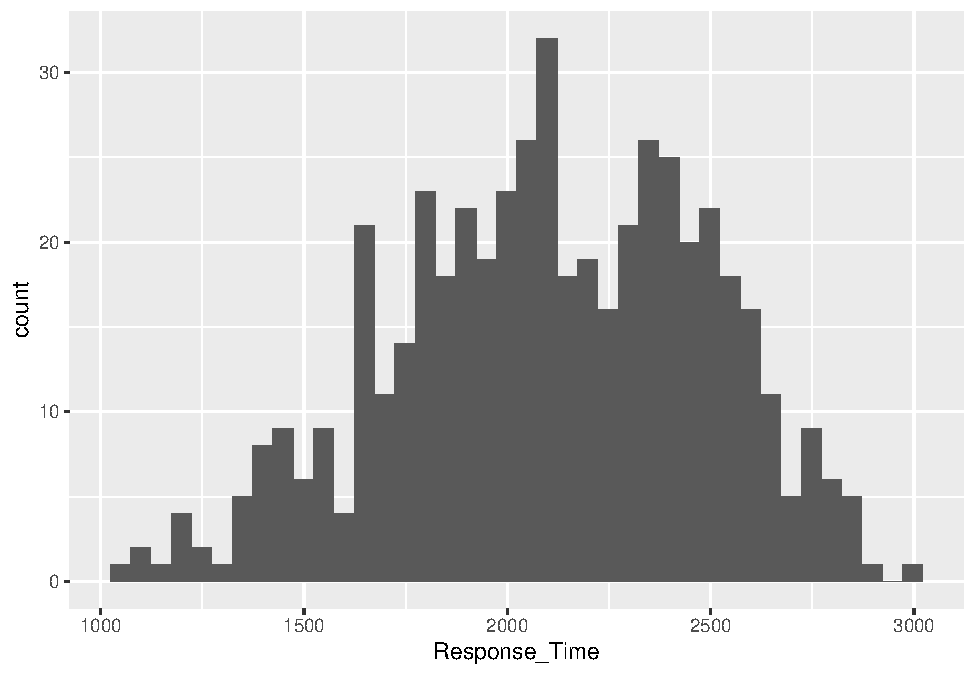
\includegraphics{Simulated_example_files/figure-latex/unnamed-chunk-7-1.pdf}
If you want to change the \texttt{stat\_bin()} you can set the argument
\texttt{bins\ =\ x} inside the \texttt{geom\_histogram()} function where
\texttt{x} is the number of bins. Note also that there are some visible
outliers in the right part of the histogram.

\begin{enumerate}
\def\labelenumi{\alph{enumi}.}
\setcounter{enumi}{5}
\tightlist
\item
  Divide the observations by the \texttt{Group} variables and fill the
  histogram with two different colors.
\end{enumerate}

\begin{Shaded}
\begin{Highlighting}[]
\FunctionTok{ggplot}\NormalTok{() }\SpecialCharTok{+} 
  \FunctionTok{geom\_histogram}\NormalTok{(}\AttributeTok{data =}\NormalTok{ db, }\FunctionTok{aes}\NormalTok{(}\AttributeTok{x =}\NormalTok{ Response\_Time,  }
                     \AttributeTok{fill =}\NormalTok{ Group), }\AttributeTok{bins=}\DecValTok{40}\NormalTok{)}\SpecialCharTok{+}
  \FunctionTok{geom\_vline}\NormalTok{(}\AttributeTok{data =}\NormalTok{ db, }\FunctionTok{aes}\NormalTok{(}\AttributeTok{xintercept =} \FunctionTok{mean}\NormalTok{(Response\_Time, }\AttributeTok{na.rm =} \ConstantTok{TRUE}\NormalTok{)),}
              \AttributeTok{linetype=}\StringTok{"dashed"}\NormalTok{, }\AttributeTok{size=}\DecValTok{1}\NormalTok{)}\SpecialCharTok{+}
  \FunctionTok{geom\_vline}\NormalTok{(}\AttributeTok{data =}\NormalTok{ db }\SpecialCharTok{\%\textgreater{}\%} \FunctionTok{filter}\NormalTok{(Group }\SpecialCharTok{==}\StringTok{"Case"}\NormalTok{), }
             \FunctionTok{aes}\NormalTok{(}\AttributeTok{xintercept=} \FunctionTok{mean}\NormalTok{(Response\_Time, }\AttributeTok{na.rm =} \ConstantTok{TRUE}\NormalTok{), }
                 \AttributeTok{colour =}\NormalTok{Group),}
             \AttributeTok{linetype=}\StringTok{"dashed"}\NormalTok{, }
             \AttributeTok{size=}\DecValTok{1}\NormalTok{)}\SpecialCharTok{+}
  \FunctionTok{geom\_vline}\NormalTok{(}\AttributeTok{data =}\NormalTok{ db }\SpecialCharTok{\%\textgreater{}\%} \FunctionTok{filter}\NormalTok{(Group }\SpecialCharTok{==}\StringTok{"Control"}\NormalTok{),}
             \FunctionTok{aes}\NormalTok{(}\AttributeTok{xintercept=}\FunctionTok{mean}\NormalTok{(Response\_Time, }\AttributeTok{na.rm =} \ConstantTok{TRUE}\NormalTok{), }
                 \AttributeTok{colour =}\NormalTok{ Group),}
             \AttributeTok{linetype=}\StringTok{"dashed"}\NormalTok{, }
             \AttributeTok{size=}\DecValTok{1}\NormalTok{)}
\end{Highlighting}
\end{Shaded}

\begin{verbatim}
## Warning: Using `size` aesthetic for lines was deprecated in ggplot2 3.4.0.
## i Please use `linewidth` instead.
## This warning is displayed once every 8 hours.
## Call `lifecycle::last_lifecycle_warnings()` to see where this warning was
## generated.
\end{verbatim}

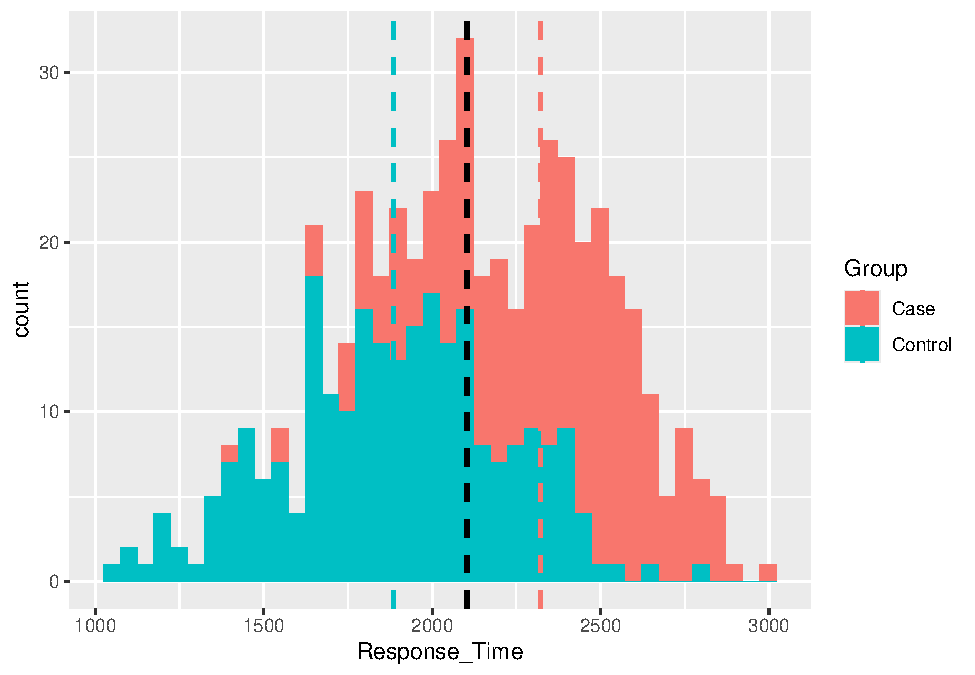
\includegraphics{Simulated_example_files/figure-latex/unnamed-chunk-8-1.pdf}

\begin{enumerate}
\def\labelenumi{\alph{enumi}.}
\setcounter{enumi}{6}
\tightlist
\item
  Generate the scatter plot between \texttt{Response\_Time} and
  \texttt{Age}, colored by Group.
\end{enumerate}

\begin{Shaded}
\begin{Highlighting}[]
\FunctionTok{ggplot}\NormalTok{(}\AttributeTok{data =}\NormalTok{ db, }
       \AttributeTok{mapping =} \FunctionTok{aes}\NormalTok{(}\AttributeTok{x =}\NormalTok{ Age, }
                     \AttributeTok{y =}\NormalTok{ Response\_Time, }
                     \AttributeTok{color =}\NormalTok{ Group)) }\SpecialCharTok{+} 
  \FunctionTok{geom\_point}\NormalTok{()}
\end{Highlighting}
\end{Shaded}

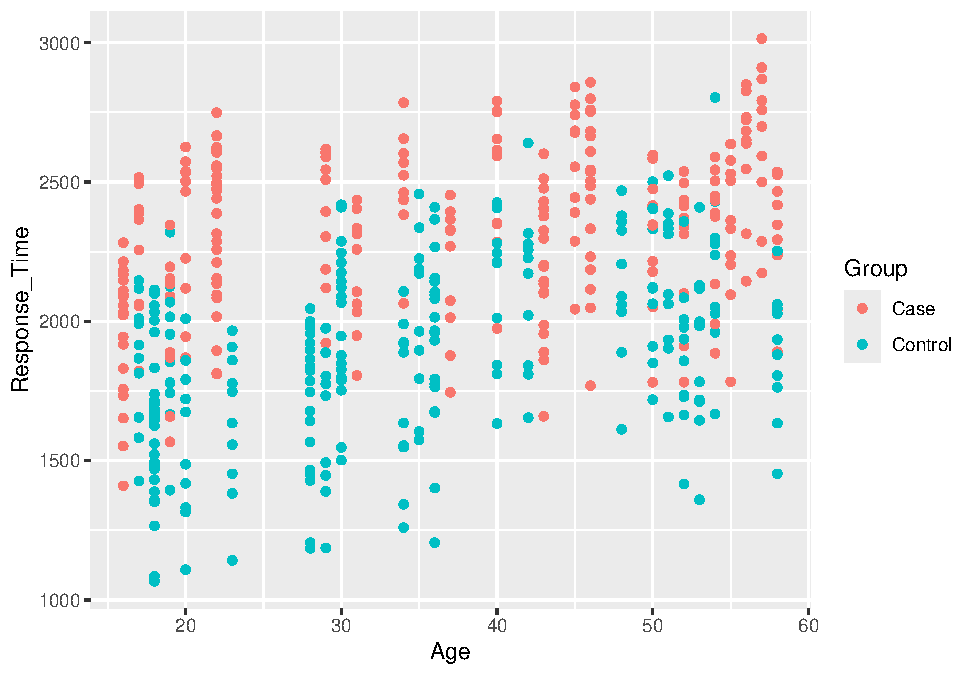
\includegraphics{Simulated_example_files/figure-latex/unnamed-chunk-9-1.pdf}
Generate another scatter dividing also by \texttt{Sex}.

\begin{Shaded}
\begin{Highlighting}[]
\FunctionTok{ggplot}\NormalTok{(}\AttributeTok{data =}\NormalTok{ db, }
       \AttributeTok{mapping =} \FunctionTok{aes}\NormalTok{(}\AttributeTok{x =}\NormalTok{ Time, }\AttributeTok{y =}\NormalTok{ Response\_Time, }\AttributeTok{color =}\NormalTok{ Group)) }\SpecialCharTok{+} 
  \FunctionTok{geom\_point}\NormalTok{() }\SpecialCharTok{+}
  \FunctionTok{facet\_wrap}\NormalTok{(. }\SpecialCharTok{\textasciitilde{}}\NormalTok{Sex)}\SpecialCharTok{+}
       \FunctionTok{scale\_colour\_discrete}\NormalTok{(}\AttributeTok{name =} \StringTok{"Group"}\NormalTok{, }\AttributeTok{labels =} \FunctionTok{c}\NormalTok{(}\StringTok{"Individuals with Alzeihmer disease"}\NormalTok{, }\StringTok{"Healthy individuals"}\NormalTok{)) }\SpecialCharTok{+}
  \FunctionTok{ylab}\NormalTok{(}\StringTok{"Response time"}\NormalTok{)}
\end{Highlighting}
\end{Shaded}

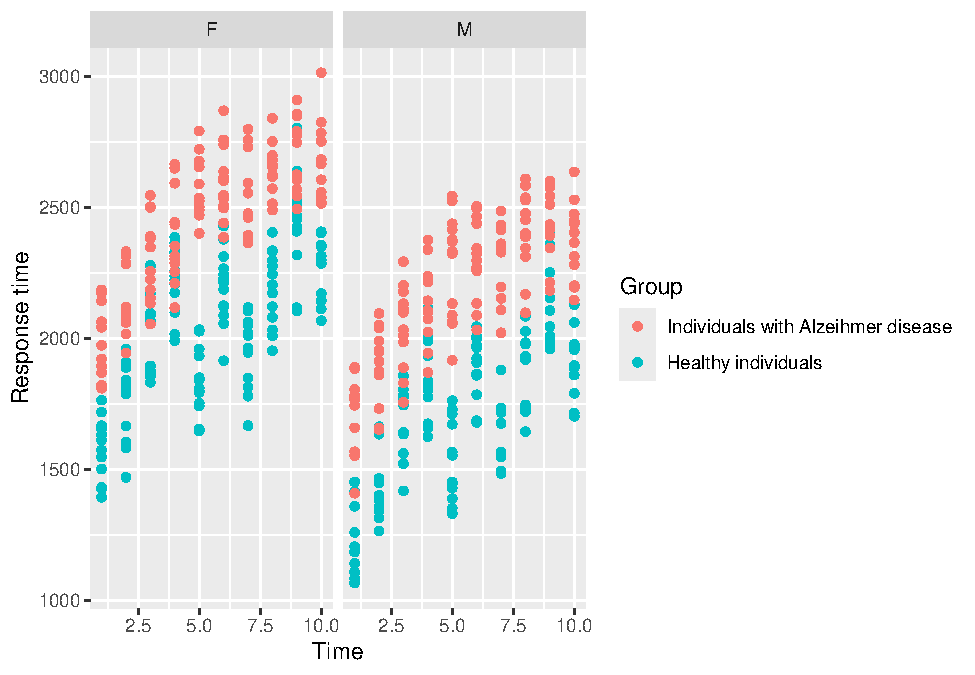
\includegraphics{Simulated_example_files/figure-latex/unnamed-chunk-10-1.pdf}
- \texttt{facet\_wrap(.\ \textasciitilde{}Sex)} - Here we put the
variable to divide the scatter plots, i.e., the Sex object. R directly
creates two plots one for each level of the Sex factor object. -
\texttt{scale\_colour\_discrete} - Here We can change the labels of the
Group legend. We must specify the name of the object as a string (i.e.,
Group) and the labels desired as vector. - \texttt{ylab} - Here We can
change the y axis.

\begin{enumerate}
\def\labelenumi{\alph{enumi}.}
\setcounter{enumi}{7}
\tightlist
\item
  Generate line plots to understand individual data
\end{enumerate}

\begin{Shaded}
\begin{Highlighting}[]
\FunctionTok{ggplot}\NormalTok{(}\AttributeTok{data =}\NormalTok{ db }\SpecialCharTok{\%\textgreater{}\%} \FunctionTok{filter}\NormalTok{(Time }\SpecialCharTok{\%in\%} \FunctionTok{c}\NormalTok{(}\DecValTok{1}\NormalTok{,}\DecValTok{5}\NormalTok{,}\DecValTok{10}\NormalTok{)), }
       \AttributeTok{mapping =} \FunctionTok{aes}\NormalTok{(}\AttributeTok{x =}\NormalTok{ Time, }\AttributeTok{y =}\NormalTok{ Response\_Time, }\AttributeTok{group =}\NormalTok{ ID, }\AttributeTok{color =}\NormalTok{ Group)) }\SpecialCharTok{+} 
  \FunctionTok{geom\_line}\NormalTok{() }\SpecialCharTok{+}
   \FunctionTok{geom\_point}\NormalTok{(}\FunctionTok{aes}\NormalTok{(}\AttributeTok{fill=}\NormalTok{Group),}
              \AttributeTok{shape=}\DecValTok{21}\NormalTok{)}
\end{Highlighting}
\end{Shaded}

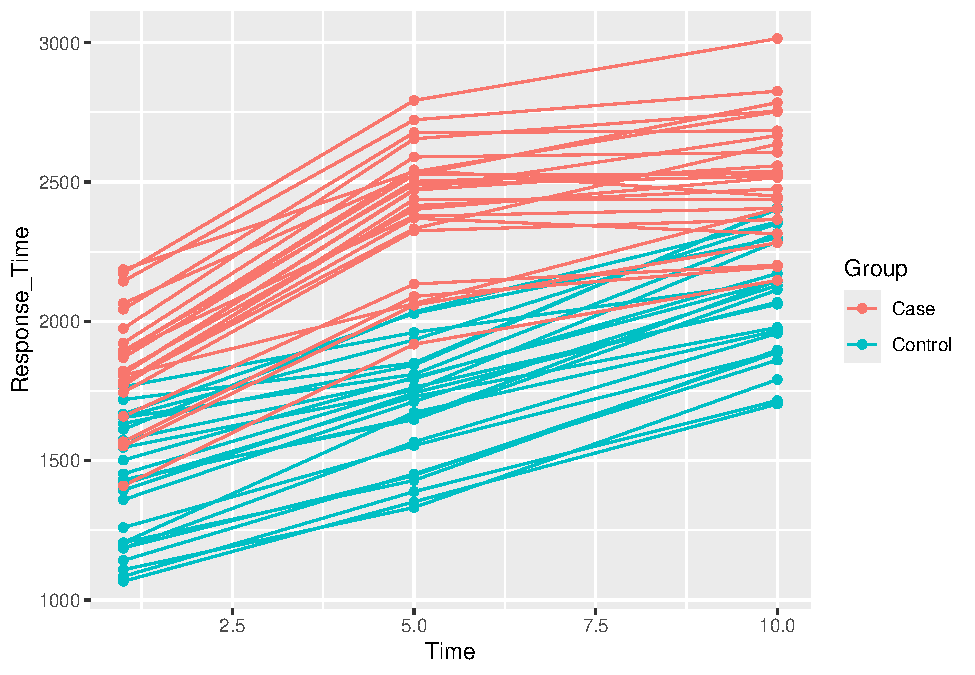
\includegraphics{Simulated_example_files/figure-latex/unnamed-chunk-11-1.pdf}
- We consider only observations at time 1, 5 and 10 -
\texttt{group\ =\ ID,\ color\ =\ Group} - Here We group the observations
by ID (i.e., one line for each individual) and We color them by
\texttt{Group}. - shape = 21 specify the type of mark (i.e., point) and
fill=Group colors the points by Group.

\begin{enumerate}
\def\labelenumi{\roman{enumi}.}
\tightlist
\item
  Plot the distribution of the \texttt{Response\_Time} variable across
  different time points (using boxplots).
\end{enumerate}

\begin{Shaded}
\begin{Highlighting}[]
\FunctionTok{ggplot}\NormalTok{(}\AttributeTok{data =}\NormalTok{ db, }
       \AttributeTok{mapping =} \FunctionTok{aes}\NormalTok{(}\AttributeTok{x =}\NormalTok{ Response\_Time, }\AttributeTok{y =}\NormalTok{ Time, }\AttributeTok{group =}\NormalTok{ Time)) }\SpecialCharTok{+} 
  \FunctionTok{geom\_boxplot}\NormalTok{() }\SpecialCharTok{+} 
  \FunctionTok{facet\_grid}\NormalTok{(. }\SpecialCharTok{\textasciitilde{}}\NormalTok{Group)}
\end{Highlighting}
\end{Shaded}

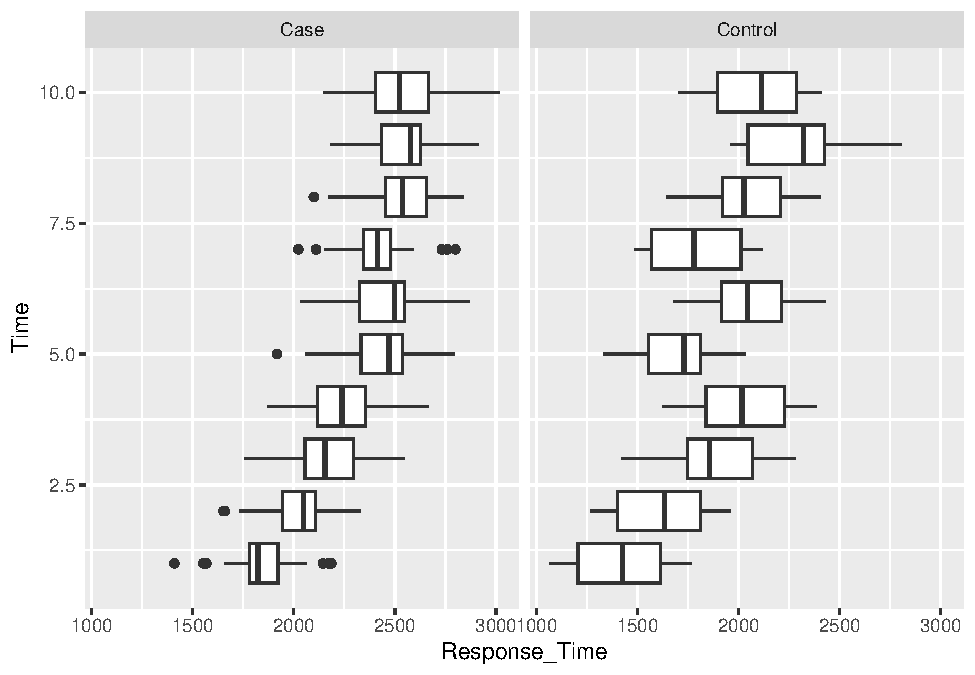
\includegraphics{Simulated_example_files/figure-latex/unnamed-chunk-12-1.pdf}

\begin{itemize}
\tightlist
\item
  \texttt{group\ =\ Time} - Here We group the observations by Time,
\item
  \texttt{facet\_grid(.\ \textasciitilde{}Group)} - We divide the plots
  into two graphs, one for the case group and one for the control
  group.\\
  Note the outliers in the right part of the graph.
\end{itemize}

\begin{enumerate}
\def\labelenumi{\alph{enumi}.}
\setcounter{enumi}{11}
\tightlist
\item
  Display the density plot of \texttt{Response\_Time} colored with
  respect to the \texttt{Group} variable.
\end{enumerate}

\begin{Shaded}
\begin{Highlighting}[]
\FunctionTok{ggplot}\NormalTok{()  }\SpecialCharTok{+}
  \FunctionTok{geom\_density}\NormalTok{(}\AttributeTok{data =}\NormalTok{ db,}
               \FunctionTok{aes}\NormalTok{(}\AttributeTok{x =}\NormalTok{ Response\_Time, }\AttributeTok{color =}\NormalTok{ Group), }\AttributeTok{size=}\DecValTok{1}\NormalTok{) }\SpecialCharTok{+}
  \FunctionTok{geom\_vline}\NormalTok{(}\AttributeTok{data =}\NormalTok{ db }\SpecialCharTok{\%\textgreater{}\%} \FunctionTok{filter}\NormalTok{(Group }\SpecialCharTok{==} \StringTok{"Case"}\NormalTok{), }
             \FunctionTok{aes}\NormalTok{(}\AttributeTok{xintercept =} \FunctionTok{mean}\NormalTok{(Response\_Time, }\AttributeTok{na.rm =} \ConstantTok{TRUE}\NormalTok{), }
                 \AttributeTok{color =}\NormalTok{ Group), }\AttributeTok{size=}\NormalTok{.}\DecValTok{8}\NormalTok{, }\AttributeTok{linetype =} \StringTok{"dotted"}\NormalTok{)}\SpecialCharTok{+}
  \FunctionTok{geom\_vline}\NormalTok{(}\AttributeTok{data =}\NormalTok{ db }\SpecialCharTok{\%\textgreater{}\%} \FunctionTok{filter}\NormalTok{(Group }\SpecialCharTok{==} \StringTok{"Control"}\NormalTok{), }
             \FunctionTok{aes}\NormalTok{(}\AttributeTok{xintercept =} \FunctionTok{mean}\NormalTok{(Response\_Time, }\AttributeTok{na.rm =} \ConstantTok{TRUE}\NormalTok{), }
                 \AttributeTok{color =}\NormalTok{ Group), }\AttributeTok{size=}\NormalTok{.}\DecValTok{8}\NormalTok{, }\AttributeTok{linetype =} \StringTok{"dotted"}\NormalTok{)}\SpecialCharTok{+}
  \FunctionTok{geom\_vline}\NormalTok{(}\AttributeTok{data =}\NormalTok{ db, }
             \FunctionTok{aes}\NormalTok{(}\AttributeTok{xintercept =} \FunctionTok{mean}\NormalTok{(Response\_Time, }\AttributeTok{na.rm =} \ConstantTok{TRUE}\NormalTok{)), }\AttributeTok{size=}\NormalTok{.}\DecValTok{8}\NormalTok{, }\AttributeTok{linetype =} \StringTok{"dashed"}\NormalTok{) }\SpecialCharTok{+}
    \FunctionTok{theme\_classic}\NormalTok{()}
\end{Highlighting}
\end{Shaded}

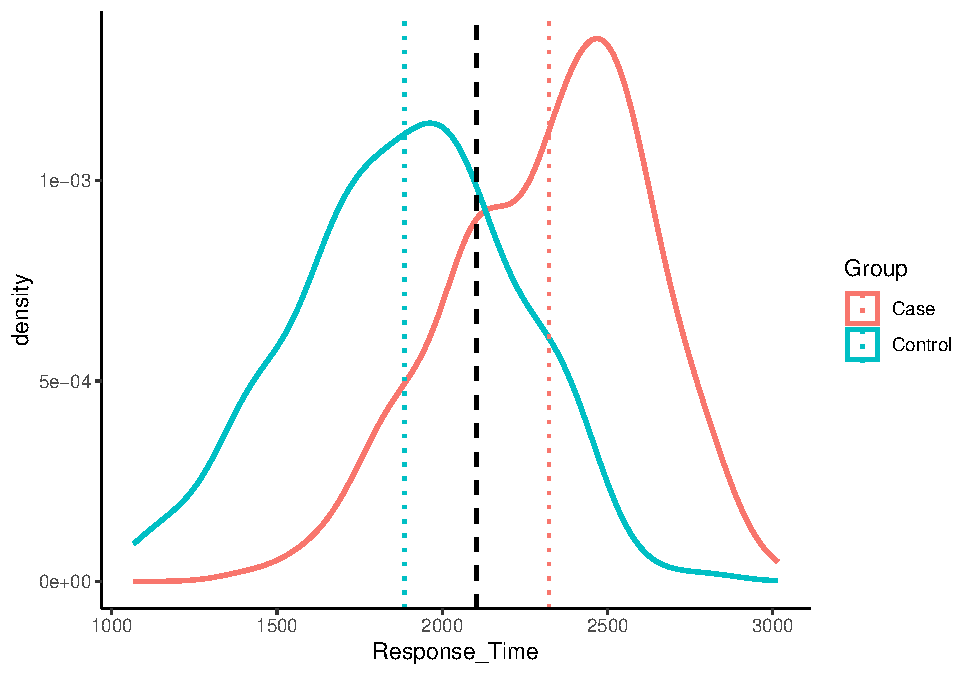
\includegraphics{Simulated_example_files/figure-latex/unnamed-chunk-13-1.pdf}

\begin{enumerate}
\def\labelenumi{\alph{enumi}.}
\setcounter{enumi}{12}
\tightlist
\item
  Display the distribution of people with respect to \texttt{Sex} and
  \texttt{Group}.
\end{enumerate}

\begin{Shaded}
\begin{Highlighting}[]
\FunctionTok{ggplot}\NormalTok{(}\AttributeTok{data =}\NormalTok{ db, }
       \AttributeTok{mapping =} \FunctionTok{aes}\NormalTok{(}\AttributeTok{x =}\NormalTok{ Group, }\AttributeTok{fill =}\NormalTok{ Sex)) }\SpecialCharTok{+} 
  \FunctionTok{geom\_bar}\NormalTok{()}
\end{Highlighting}
\end{Shaded}

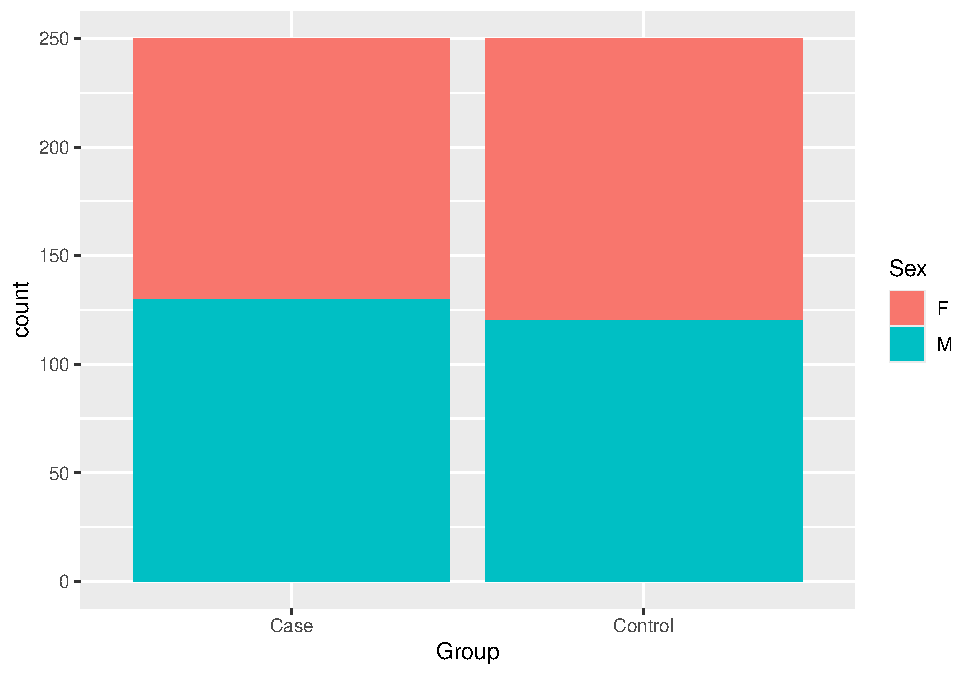
\includegraphics{Simulated_example_files/figure-latex/unnamed-chunk-14-1.pdf}

\begin{enumerate}
\def\labelenumi{\alph{enumi}.}
\setcounter{enumi}{13}
\tightlist
\item
  check the correlation between the quantitative variables and Plot the
  correlation matrix.
\end{enumerate}

\begin{Shaded}
\begin{Highlighting}[]
\NormalTok{corr\_matrix }\OtherTok{\textless{}{-}} \FunctionTok{round}\NormalTok{(}\FunctionTok{cor}\NormalTok{(db[,}\SpecialCharTok{!}\NormalTok{(}\FunctionTok{colnames}\NormalTok{(db) }\SpecialCharTok{\%in\%} \FunctionTok{c}\NormalTok{(}\StringTok{"Sex"}\NormalTok{, }\StringTok{"Group"}\NormalTok{, }\StringTok{"ID"}\NormalTok{))], }\AttributeTok{use =} \StringTok{"complete.obs"}\NormalTok{), }\DecValTok{2}\NormalTok{)}
\NormalTok{corr\_matrix[}\FunctionTok{lower.tri}\NormalTok{(corr\_matrix)] }\OtherTok{\textless{}{-}} \DecValTok{0}
\NormalTok{corr\_matrix}
\end{Highlighting}
\end{Shaded}

\begin{verbatim}
##               Age ATTC1 Response_Time Time
## Age             1  0.05          0.35 0.00
## ATTC1           0  1.00          0.61 0.13
## Response_Time   0  0.00          1.00 0.53
## Time            0  0.00          0.00 1.00
\end{verbatim}

\begin{Shaded}
\begin{Highlighting}[]
\FunctionTok{library}\NormalTok{(ggcorrplot)                                             }
\end{Highlighting}
\end{Shaded}

\begin{verbatim}
## Warning: il pacchetto 'ggcorrplot' è stato creato con R versione 4.3.3
\end{verbatim}

\begin{Shaded}
\begin{Highlighting}[]
\FunctionTok{ggcorrplot}\NormalTok{(corr\_matrix, }
           \AttributeTok{type =} \StringTok{"upper"}\NormalTok{, }
           \AttributeTok{lab =}\NormalTok{ T, }
           \AttributeTok{lab\_size =} \DecValTok{7}\NormalTok{, }
           \AttributeTok{outline.col =} \StringTok{"white"}\NormalTok{, }
           \AttributeTok{colors =} \FunctionTok{c}\NormalTok{(}\StringTok{"tomato2"}\NormalTok{, }\StringTok{"white"}\NormalTok{, }\StringTok{"springgreen3"}\NormalTok{), }
           \AttributeTok{title =} \StringTok{""}\NormalTok{, }
           \AttributeTok{ggtheme =}\NormalTok{ theme\_gray, }
           \AttributeTok{pch.cex =} \DecValTok{30}\NormalTok{, }
           \AttributeTok{tl.cex =} \DecValTok{20}\NormalTok{)}
\end{Highlighting}
\end{Shaded}

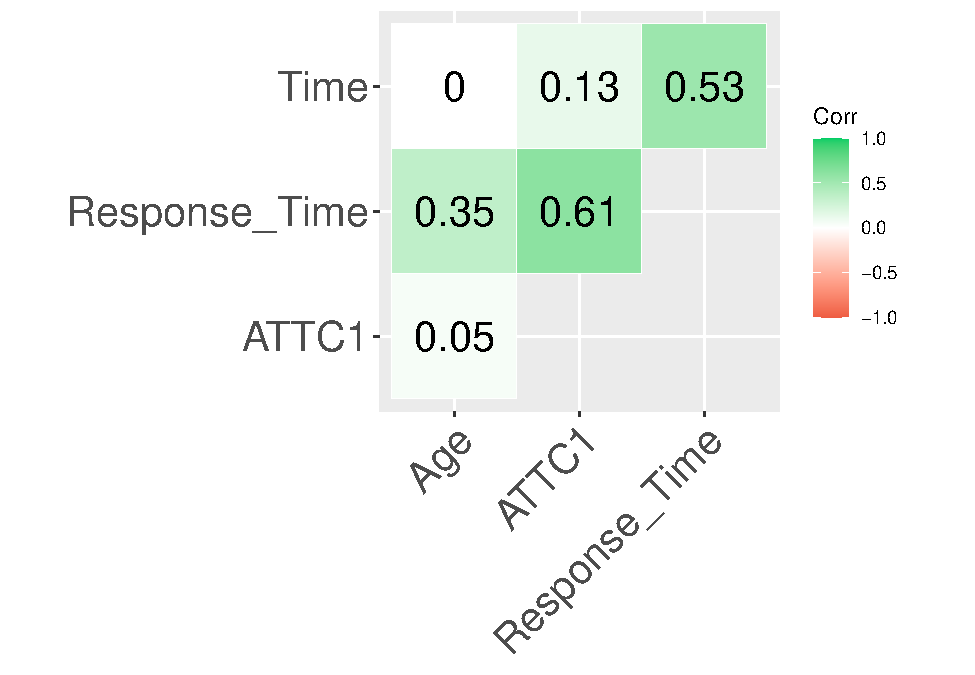
\includegraphics{Simulated_example_files/figure-latex/unnamed-chunk-15-1.pdf}

\begin{enumerate}
\def\labelenumi{\alph{enumi}.}
\setcounter{enumi}{14}
\tightlist
\item
  Remove observations with NA
\end{enumerate}

\begin{Shaded}
\begin{Highlighting}[]
\NormalTok{db }\OtherTok{\textless{}{-}}\NormalTok{ db }\SpecialCharTok{\%\textgreater{}\%} \FunctionTok{filter}\NormalTok{(}\SpecialCharTok{!}\FunctionTok{is.na}\NormalTok{(Response\_Time))}
\CommentTok{\# Alternatively, we can use the basic commands of R:}
\CommentTok{\#db \textless{}{-} db[!is.na(db$Response\_Time),]}
\end{Highlighting}
\end{Shaded}

\begin{enumerate}
\def\labelenumi{\alph{enumi}.}
\setcounter{enumi}{15}
\tightlist
\item
  Ideas for other plots?
\end{enumerate}

\end{document}
